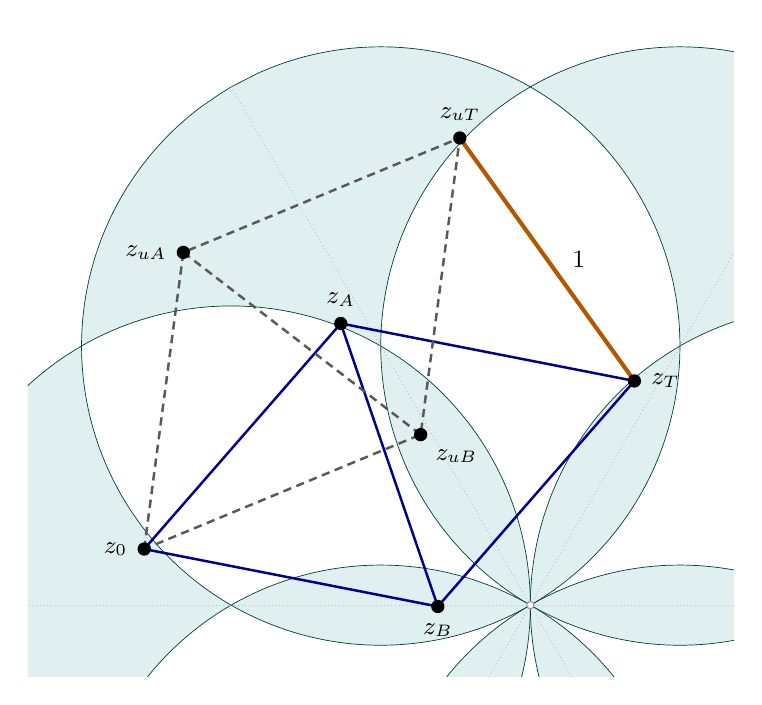
\begin{tikzpicture}[x=3.8cm,y=3.8cm,font=\small,
  vertex/.style={circle,fill=black,inner sep=1.7pt},
  first/.style={blue!55!black,line width=.9pt},
  second/.style={black!65,line width=.9pt,densely dashed}]
  \begin{scope}
    \clip (-1.68,-.24) rectangle (.68,1.93);
    \foreach \sector in {0,60,120,180,240,300} {
      \path[fill=teal!12,draw=teal!45!black,line width=.25pt]
        plot[domain=0:1,samples=101,variable=\r]
          ({\r*cos(\sector+acos(\r/2)-60)},
           {\r*sin(\sector+acos(\r/2)-60)})
        -- plot[domain=1:0,samples=101,variable=\r]
          ({\r*cos(\sector-acos(\r/2)+60)},
           {\r*sin(\sector-acos(\r/2)+60)}) -- cycle;
      \path[fill=teal!12,draw=teal!45!black,line width=.25pt]
        plot[domain=1:sqrt(3),samples=101,variable=\r]
          ({\r*cos(\sector+60-acos(\r/2))},
           {\r*sin(\sector+60-acos(\r/2))})
        -- plot[domain=sqrt(3):2,samples=101,variable=\r]
          ({\r*cos(\sector+acos(\r/2))},
           {\r*sin(\sector+acos(\r/2))})
        -- plot[domain=2:sqrt(3),samples=101,variable=\r]
          ({\r*cos(\sector-acos(\r/2))},
           {\r*sin(\sector-acos(\r/2))})
        -- plot[domain=sqrt(3):1,samples=101,variable=\r]
          ({\r*cos(\sector-60+acos(\r/2))},
           {\r*sin(\sector-60+acos(\r/2))}) -- cycle;
    }
    \foreach \sector in {0,60,120,180,240,300}
      \draw[black!25,densely dotted,line width=.35pt]
        (0,0) -- (\sector:2);
    \draw[fill=white,draw=black!45,line width=.3pt]
      (0,0) circle[radius=.012];
  \end{scope}
  \foreach \name/\gx/\gy in {
    O/0/0,
    A/{sqrt(3)/2}/{1/2},
    B/{sqrt(3)/2}/{-1/2},
    T/{sqrt(3)}/0,
    UA/{(5*sqrt(3)-sqrt(11))/12}/{(sqrt(33)+5)/12},
    UB/{(5*sqrt(3)+sqrt(11))/12}/{(sqrt(33)-5)/12},
    UT/{5*sqrt(3)/6}/{sqrt(33)/6}}
  {
    \coordinate (\name) at
      ({(35*(\gx-290/250)-12*(\gy+149/250))/37},
       {(12*(\gx-290/250)+35*(\gy+149/250))/37});
  }
  \draw[first] (O) -- (A) -- (T) -- (B) -- (O);
  \draw[first] (A) -- (B);
  \draw[second] (O) -- (UA) -- (UT) -- (UB) -- (O);
  \draw[second] (UA) -- (UB);
  \draw[orange!70!black,line width=1.5pt] (T) --
    node[midway,right=5pt,text=black] {$1$} (UT);

  \node[vertex,label=left:$z_0$] at (O) {};
  \node[vertex,label=above:$z_A$] at (A) {};
  \node[vertex,label=below:$z_B$] at (B) {};
  \node[vertex,label=right:$z_T$] at (T) {};
  \node[vertex,label=left:$z_{uA}$] at (UA) {};
  \node[vertex,label=below right:$z_{uB}$] at (UB) {};
  \node[vertex,label=above:$z_{uT}$] at (UT) {};
\end{tikzpicture}
